\subsection{Pipeline Parallelism}
\label{section:pp}

When using a BF16 number representation for the model parameters, \llamathree 405B does not fit in the GPU memory of a single machine with 8 Nvidia H100 GPUs. 
To address this issue, we parallelize model inference using BF16 precision across 16 GPUs on two machines.
Within each machine, the high NVLink bandwidth enables the use of tensor parallelism \citep{shoeybi2019megatron}. 
Across nodes, however, connectivity has lower bandwidth and higher latency, so we use pipeline parallelism \citep{huang2019gpipe} instead.

During training with pipeline parallelism, bubbles are a major efficiency concern (see Section~\ref{section:pretraining_model_scaling}).
However, they are not an issue during inference, since inference does not involve a backward pass that requires a pipeline flush. 
Therefore, we use micro-batching to improve inference throughput with pipeline parallelism. 

We evaluate the effect of using two micro-batches in inference workloads of 4,096 input tokens and 256 output tokens both during the key-value cache \emph{pre-fill} stage of inference and during the \emph{decoding} stage.
We find that micro-batching improves throughput of inference with the same local batch size; see Figure~\ref{figure:micro-batching}.
These improvements result from micro-batching enabling concurrent execution of micro batches in both these stages.
The additional synchronization points due to micro-batching also increase latency but, overall, micro-batching still leads to a better throughput-latency trade-off.

\begin{figure}
\centering
\begin{subfigure}{.5\textwidth}
  \centering
  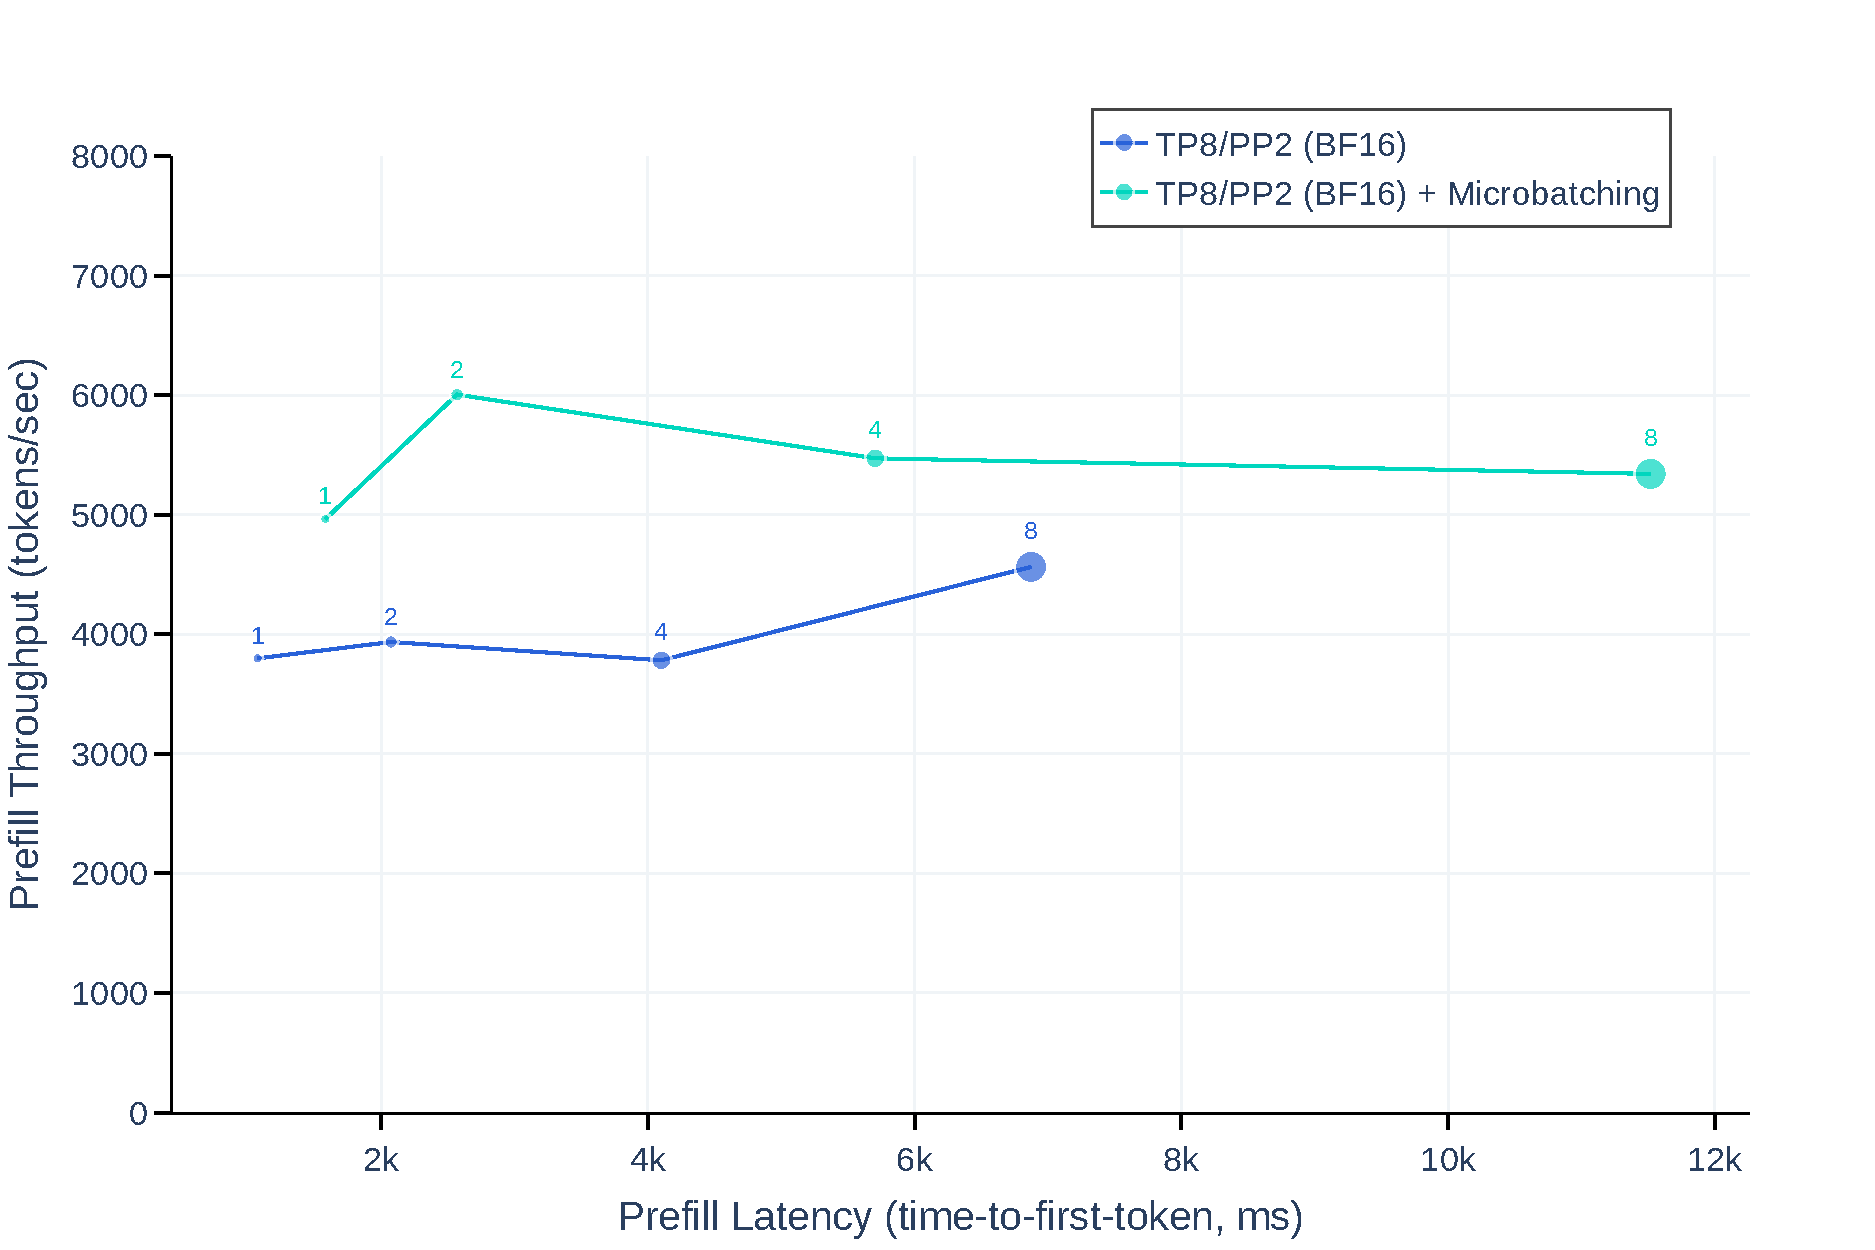
\includegraphics[width=\linewidth]{assets/prefill_micro.pdf}
\end{subfigure}%
\begin{subfigure}{.5\textwidth}
  \centering
  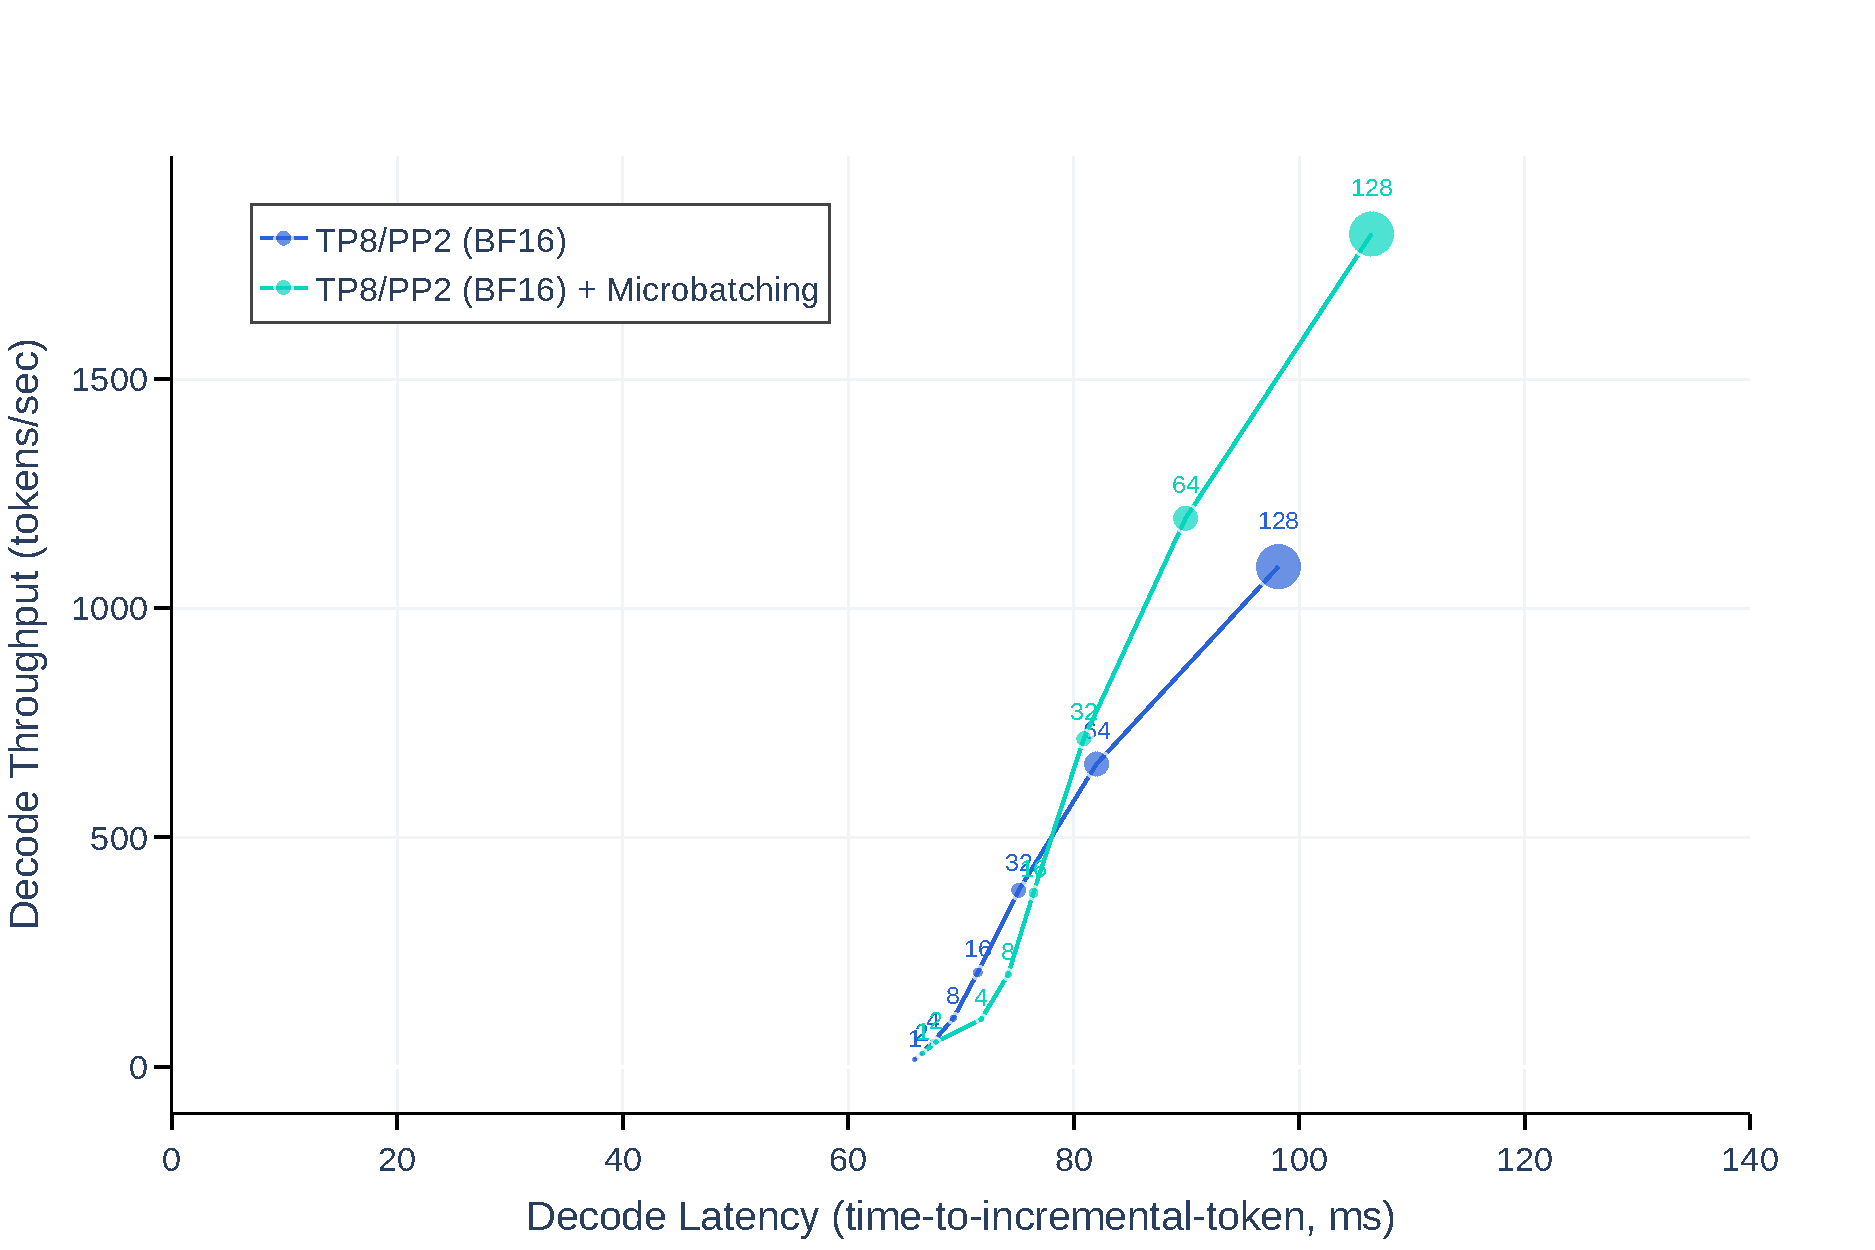
\includegraphics[width=\linewidth]{assets/decode_micro.pdf}
\end{subfigure}
\caption{\textbf{Effect of micro-batching on inference throughput and latency} during the \emph{Left:} pre-filling and \emph{Right:} decoding stage. The numbers in the plot correspond to the (micro-)batch size.}

\label{figure:micro-batching}
\end{figure}


